\chapter{Conclusioni} \label{cap3}
\def\baselinestretch{1.66}
\section{Database}
Il database mostrato di seguito \`e usato per conservare le informazioni di accesso degli
amministratori, i prodotti da vendere, gli acquisti delle bibite e le chiavi ricaricabili.
Quest'ultime sono le uniche che contengono informazioni sugli utenti, poich\`e a seguito di assunzioni
si \`e pensato che gli utenti vengano registrati dal DBA, cos\`i come gli amministratori. A
seguito di ci\`o nello sviluppo non \`e stato preso in considerazione una pagina per la registrazione e un metodo nella classe Dao per l'eliminazioni di tuple.

\begin{figure}[ht]
    \centering
    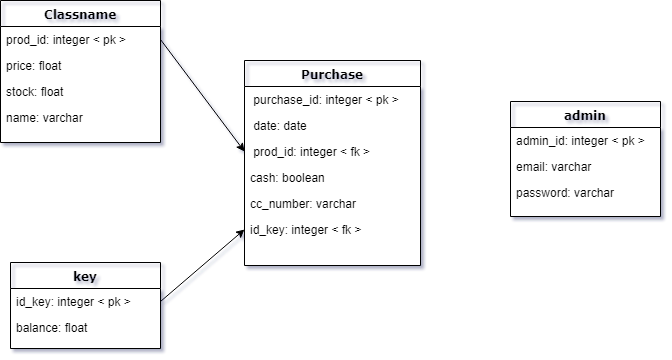
\includegraphics[scale=0.5]{img/database.png}
    \caption{Database relazionale.}
\end{figure}
